\newpage
\subsection{The communication protocol definition}
\label{subsec:communication} 

\vspace{0.5cm}
\begin{bytefield}[endianness=little, bitwidth=2.4em]{16}
    \begin{rightwordgroup}{Header}
        \bitheader[lsb=0]{0-15} \\
        \bitbox{1}{STX}
        \bitbox{4}{LENGTH}
        \bitbox{1}{RS}
        \bitbox{4}{DEST}
        \bitbox{1}{RS}
        \bitbox{4}{SOURCE}
        \bitbox{1}{RS}
    \end{rightwordgroup}
    \\ \\
    \begin{rightwordgroup}{Body}
        \bitheader[lsb=16]{16-20} \\
        \bitbox{4}{MSG\_ID}
        \bitbox{1}{RS}
        \bitbox{1}{PC}
        \bitbox{1}{US}
        \bitbox{2}{PAR 1}
        \bitbox{1}{US}
        \bitbox{2}{...}
        \bitbox{1}{US}
        \bitbox{2}{PAR n}
        \bitbox{1}{EOT}
    \end{rightwordgroup}
\end{bytefield}
\vspace{0.5cm}

\noindent
In this first section, the basic standards applied to each message within the communication protocol will be presented. Each data/info exchange between different actors of the system is required to be constructed following those same rule. The result will be a working communication channel for the required application between different modules.

\medskip The diagram above shows the standard composition of a message. Reference numbers have been defined to locate the character position of elements within the not-variable portion of the message. The structure is defined with the support of four ASCII control character: STX (Start of text), EOT (End of transmission), RS (Record separator) and US (Unit separator). Each message must start with the control character STX and end with EOT. This rule delimits the boundaries for each message both client and Server can retrieve from the communication stream. Basic correctness checking could be then implemented by testing these rules on both hands of the channel. The message is substantially made of a sequence of \textbf{records}, each separated from the others by the character RS. Each record contains inside data that is always expressed in Big Endian with reference to the diagram (i.e. the least significant digit of LENGTH is at the 4th character of the message). Records that contain different pieces of data are partitioned in \textbf{units}, each separated by the character US. For example, the last record of the message structure contains the optional parameters that are partitioned in different units for each particular parameter (plus a unit containing the count of parameters inside the message).

\medskip Inside each message it is possible to identify a \textbf{Header} and a \textbf{Body}. The former is extremely static, having a fixed length (16 bytes) and fixed number of records. The Body, on the other hand, contains both a record indicating the kind of message (MSG\_ID) and therefore is fixed in length up to this point, but can be extended with a variable number of parameters to follow. Generally speaking, messages can be found in either one of the following forms.

\vspace{0.5cm}
\begin{bytefield}[endianness=little, bitwidth=2.4em]{16}
    \bitbox{2}{Header}
    \bitbox{4}{MSG\_ID}
    \bitbox{1}{EOT}
    \\ \\
    \bitbox{2}{Header}
    \bitbox{4}{MSG\_ID}
    \bitbox{1}{RS}
    \bitbox{1}{PC}
    \bitbox{1}{US}
    \bitbox{4}{parameter units}
    \bitbox{1}{EOT}
\end{bytefield}
\vspace{0.5cm}

\medskip While the Header can be easily described and implemented, the Body requires an in-depth description of every single function. A list of all defined body-description can be found in the appendix which illustrates each possible MSG\_ID and how it can be built (with or without parameters) for any occurring event (see appendix \ref{appendix:messages_list}). In the following page, a table containing a description of each record/unit is presented as well.

\begin{table}[H]
\centering
\caption{Description of components within a message}
\label{my-label}
\begin{tabular}{|l|l|l|p{10cm}|}
\hline
\textbf{Field} & \textbf{Type} & \textbf{Length} & \textbf{Description}  \\ \hline
STX            & c             & 1               & Byte used to indicate the beginning of any new message. It is represented with the ASCII code 2, the "start of text" character \newline \\
RS             & c             & 1               & Byte used to indicate the separation between two record structures. It is represented with the ASCII code 30, the "record separator" charachter \newline \\
US             & c             & 1               & Byte used to indicate the separation between two unit structures (inside a record). It is represented with the ASCII code 31, the "unit separator" charachter \newline \\
EOT            & c             & 1               & Byte used to indicate the end of any new message. It is presented with the ASCII code 4, the "end of transmission" character \newline \\
LENGTH         & d             & 4               & Record describing the length of the whole message, from STX to EOT included \newline \\
DEST           & d             & 4               & Record describing the unique identifier of the destination. Each identifier is an alphanumeric code composed of a letter (S for server, P for plush toy and U for users on mobile APP) followed by a numeric code \newline \\
SOURCE         & d             & 4               & Record describing the unique identifier of the source. The identifier is defined in the same way as for the destination record \newline \\
MSG\_ID        & d             & 4               & Record describing the content of the message itself via a unique numeric identifier \newline \\ 
PC             & d             & 1               & Byte containing the number of optional parameters contained in the message (without counting PC itself) \newline \\
PAR x          & d             & variable        & Each parameter unit describes a piece of data specific of the message sent. The length is variable as well. Each parameter is divided by a US separator \\ \hline
\end{tabular}
\end{table}
\label{tab:comm_message}

\textbf{Type}

c : ASCII control character, no useful information but required for the structure

d : data record/unit containing useful information of the message

\newpage
The communication protocol has been designed such that the server would act as the middleman between plush toys and Android users. Each interaction between clients will be parsed by the server, which will redirect received messages to the right destination. This design choice brings two main benefits to the system: firstly, each communication is checked for correctness by the server, protecting clients from vulnerability due to bad-constructed messages; secondly, this design introduces a higher level of abstraction for each client, which are not required to deal with networking details (IP address, ports, etc).

\medskip
An example of such abstraction could be illustrated with the so-called "introduction message", labelled with MSG\_ID equal to 0001 (see appendix \ref{appendix:messages_list} for reference). The following illustration represents an example of an introduction message a plush toy could construct upon connecting to the server. In fact, following the protocol, each client is required to send a message to the server (labeled S001 in the example) which contains the MSG\_ID record equal to 0001, as well as the the SOURCE record set to the unique identifier of the client itself. This operation is necessary as we aim to have an environment for which messages sent between clients do not require any networking related information (IP address and port), but could only rely on identifiers (P314, U123).

\begin{center}
    \begin{bytefield}[endianness=little, bitwidth=2.4em]{16}
        \bitbox{1}{STX}
        \bitbox{2}{20}
        \bitbox{1}{RS}
        \bitbox{2}{S001}
        \bitbox{1}{RS}
        \bitbox{2}{P314}
        \bitbox{1}{RS}
        \bitbox{2}{0001}
        \bitbox{1}{EOT}
    \end{bytefield}
\end{center}

The described protocol encourages such abstract identifiers associated with each client (and server). Therefore, upon connecting to the server, clients are supposed to identify themselves with the "introduction message" which will allow a direct matching between the abstraction (P314) and their current network information (xyz.jkw.abc.def), transparent to all actors in the system.

\subsubsection{An example pipeline}
In order to provide a clear description of the adoption of such communication protocol, figure \ref{fig:SE_sequenceDiag} on the following page illustrates a possible pipeline between three actors. The communication is held by a Server (labeled S001) and two clients, a plush toy (P314) and a parent as Android user (U123). The diagram presented has been created by following the UML standard for sequence diagrams.

\medskip
The diagram in figure \ref{fig:SE_sequenceDiag}(a) illustrates message exchanges during the pairing procedure between a parent APP and a toy. To such intent, the parent log-in via the application by typing both required user-name and password. Such information is sent to the server, which will alternatively return either the user identifier or an error code (see appendix \ref{appendix:messages_list}). At this stage, the parent will request to the toy the "pairing privilege". This latter is required to accept such request (for security reasons) by interacting with the touch sensors. If a successful result is obtained before a set timeout, the parent and the toy are associated together and will be able to interact in the future.

\medskip
Finally, the diagram in figure \ref{fig:SE_sequenceDiag}(b) showcases trivial interchanges of messages during a playing session. Parents can initiate a session, which is then accepted by the child by playing with the toy. At this stage, both parent and child can interact with each other by turning on/off LEDs and playing sounds at each end of the channel.

\bigskip
\noindent
\textbf{N.B.} Messages in both diagrams are indicated as "MSG\_ID | PAR\_1 | PAR\_2" for simplicity

\begin{sidewaysfigure}
    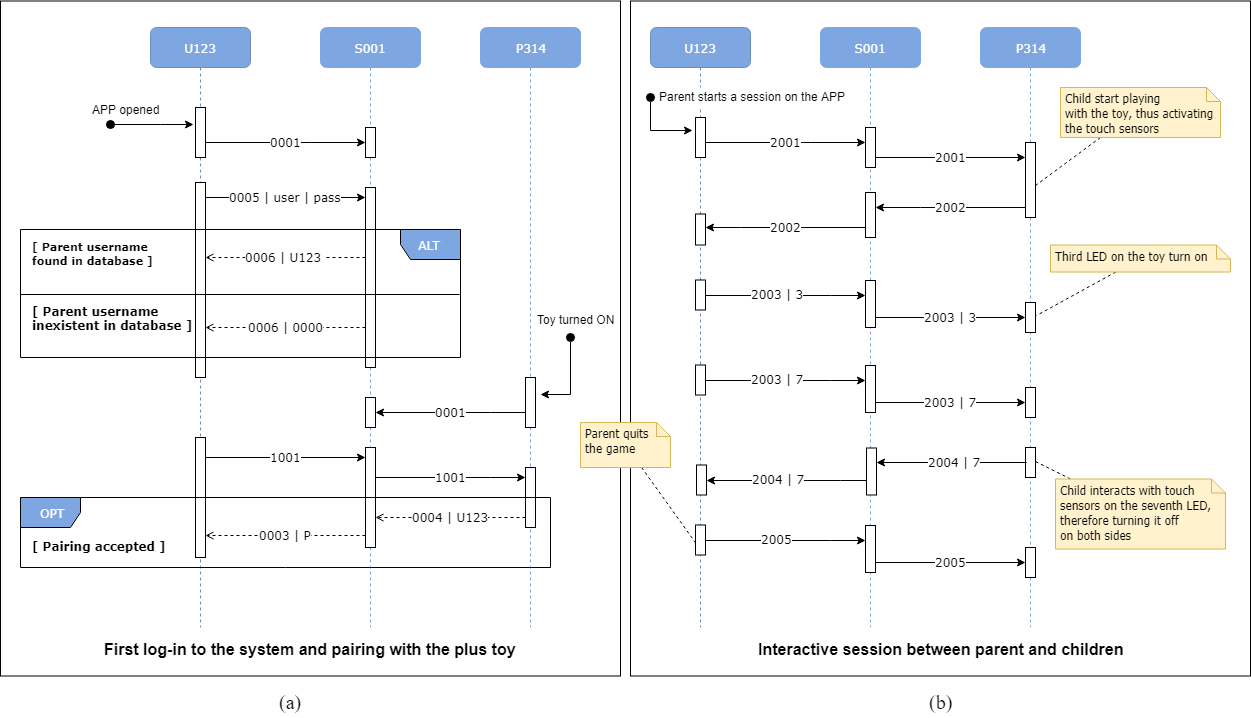
\includegraphics[scale=0.58]{images/SE_communication_sequence.png}
    \caption{UML Sequence diagram for a communication pipeline example}
    \label{fig:SE_sequenceDiag}
\end{sidewaysfigure}